\documentclass[xetex]{beamer}

\usepackage[english]{babel}
\usepackage{polyglossia}
\setdefaultlanguage{french}
\usepackage{graphicx}
\usepackage{adjustbox}
\usepackage{tikz, pgfplots}
\usetheme{modern}


\title
    {Architecture des systèmes d'information}
\subtitle
    {Gestion des contacts d'une banque}
\author
    {H4401}


\begin{document}

    \frame[plain]{\titlepage}

    \frame{\tableofcontents}

    \section{Découpage MCD et objets métier (Antoine)}
     \begin{frame}{Découpage MCD (1)}
	
\noindent\makebox[\textwidth]{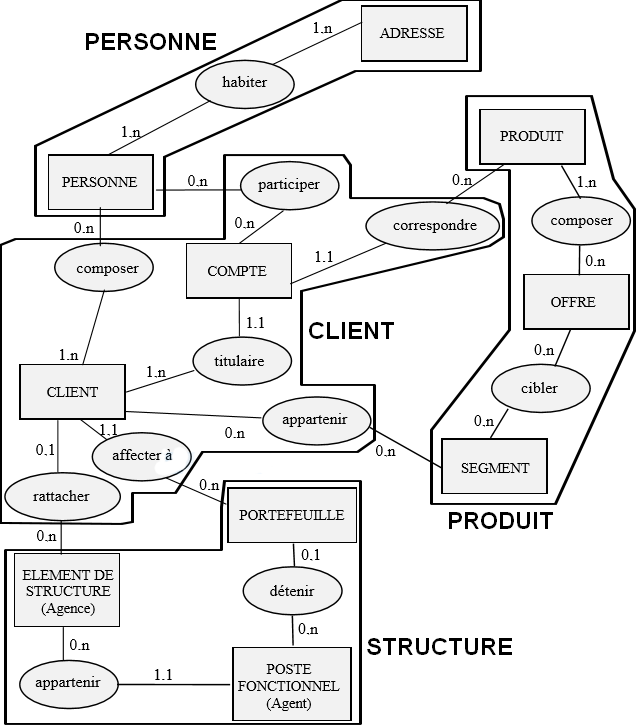
\includegraphics[height=8cm]{../report/figures/mcd/MCD_Clients_Produits.png}}

    \end{frame}
    \begin{frame}{Découpage MCD (2)}
\noindent\makebox[\textwidth]{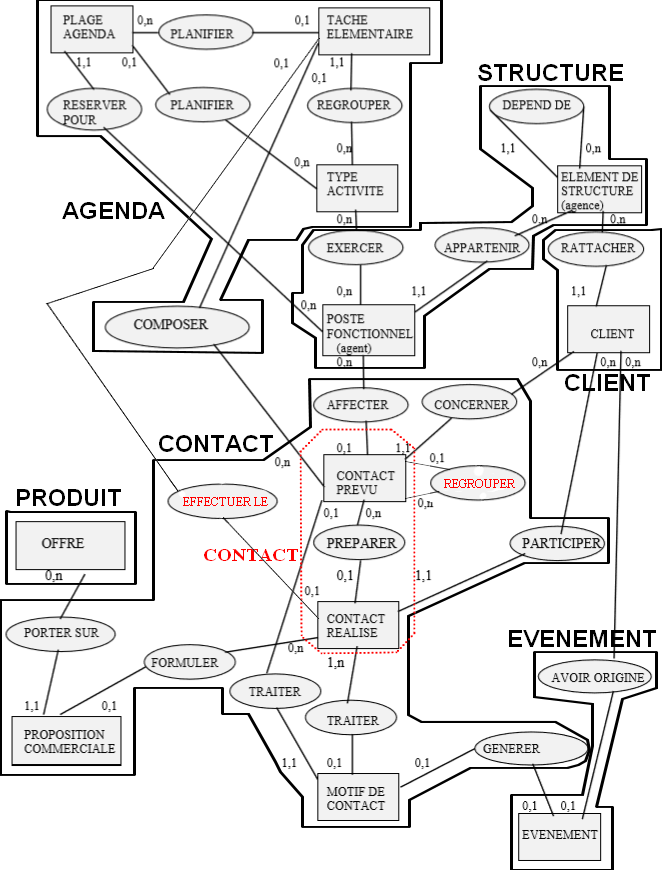
\includegraphics[height=8cm]{../report/figures/mcd/MCD_Commercial.png}}
    \end{frame}
    \section{Diagramme d’état (Paul)}
    \begin{frame}{Diagramme d'état de l'objet contact}
\noindent\makebox[\textwidth]{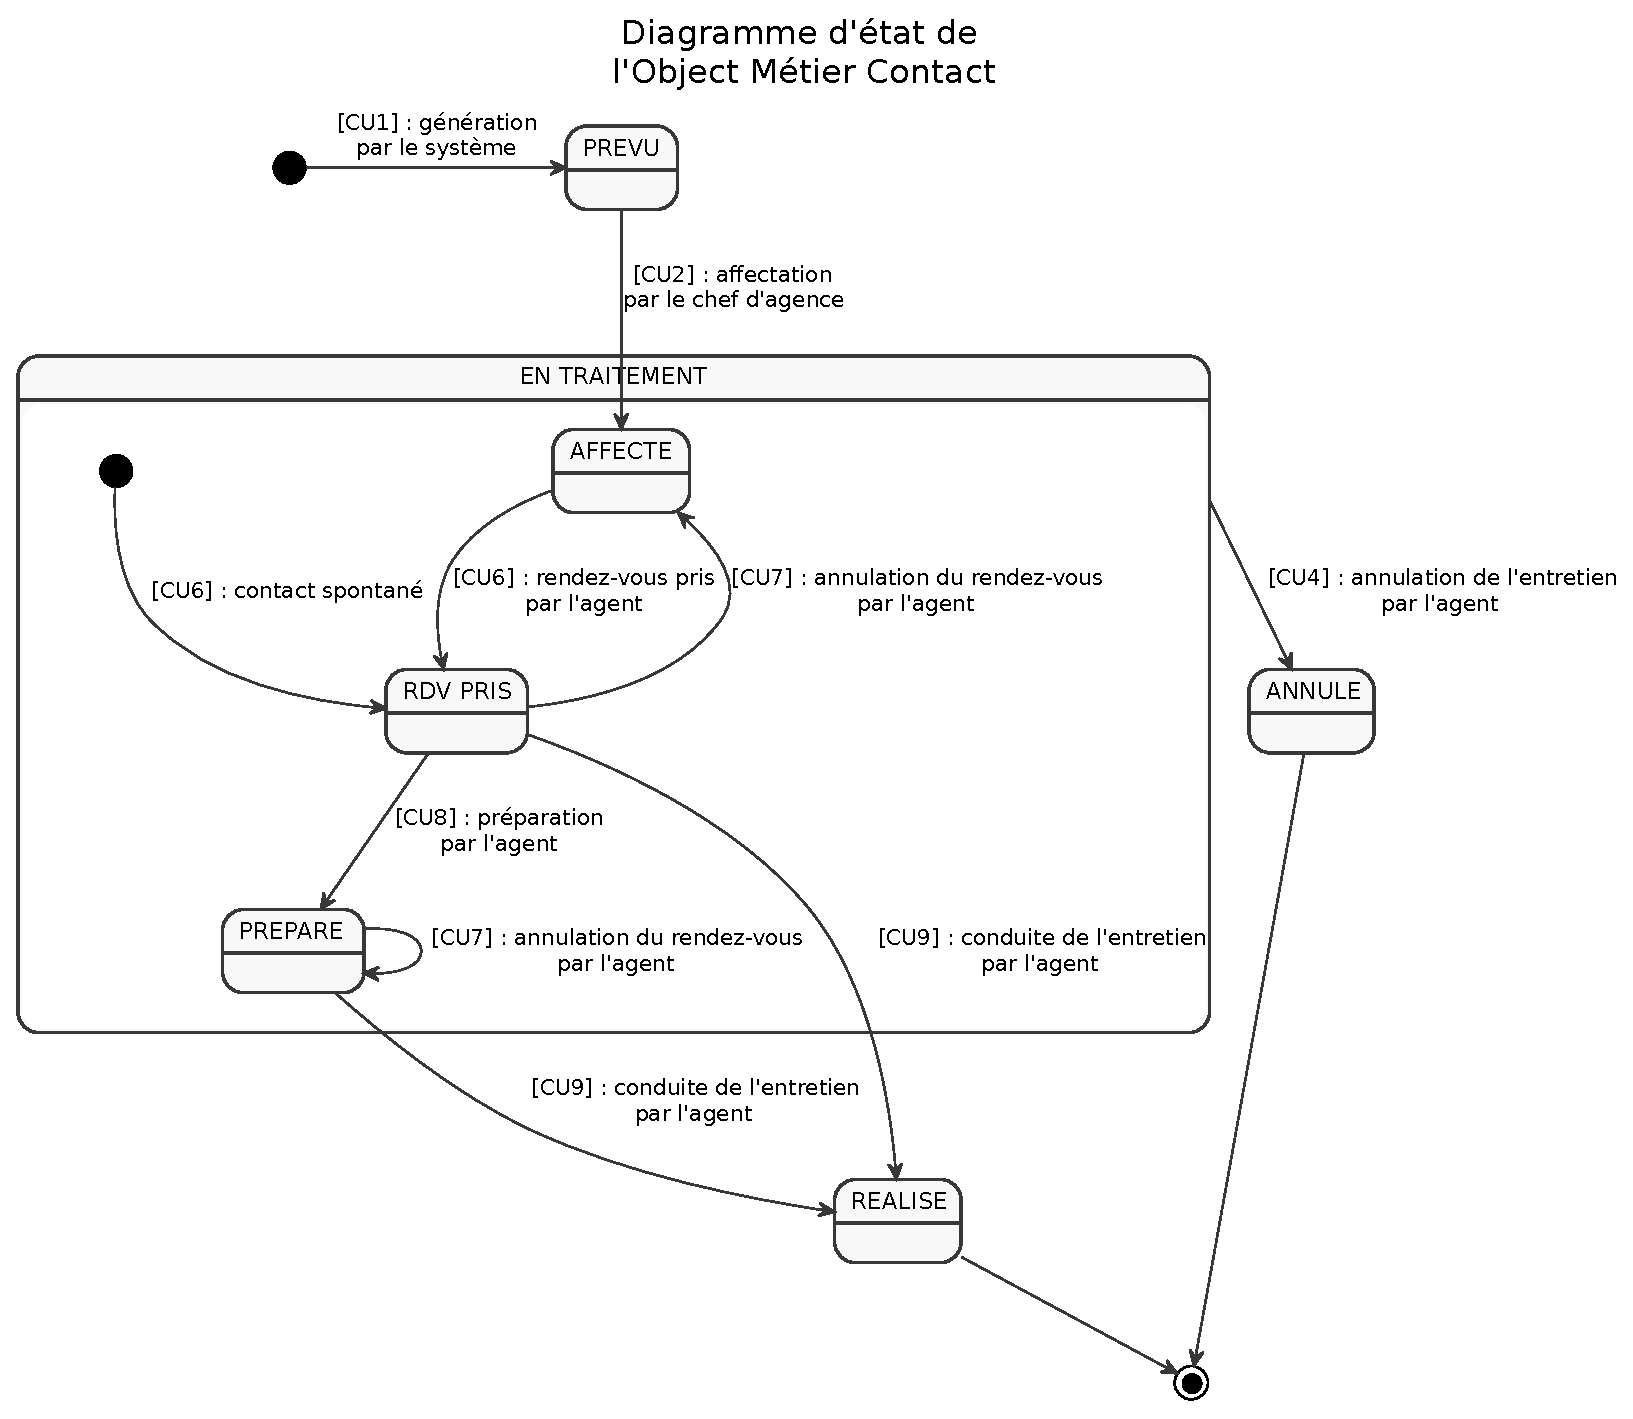
\includegraphics[height=8cm]{../report/figures/eps/diag_etats_contact}}
    \end{frame}
    \section{IHM Agenda (Hugues)}

 \begingroup
        \setbeamercolor{background canvas}{parent=palette secondary}
        \begin{frame}[plain]
            \centering
            \vfill
            \usebeamerfont{section title}\usebeamercolor[fg]{frametitle}IHM Agenda
            \vfill
        \end{frame}
    \endgroup    
    
    \section{Diagramme de séquence détaillé - CU7 (Lisa)}
    \begin{frame}{Diagramme de séquence détaillé - CU7}
    \adjustbox{width=1.1\textwidth, center, trim={0} {.45\height} {0} {0.15cm},clip}%
  {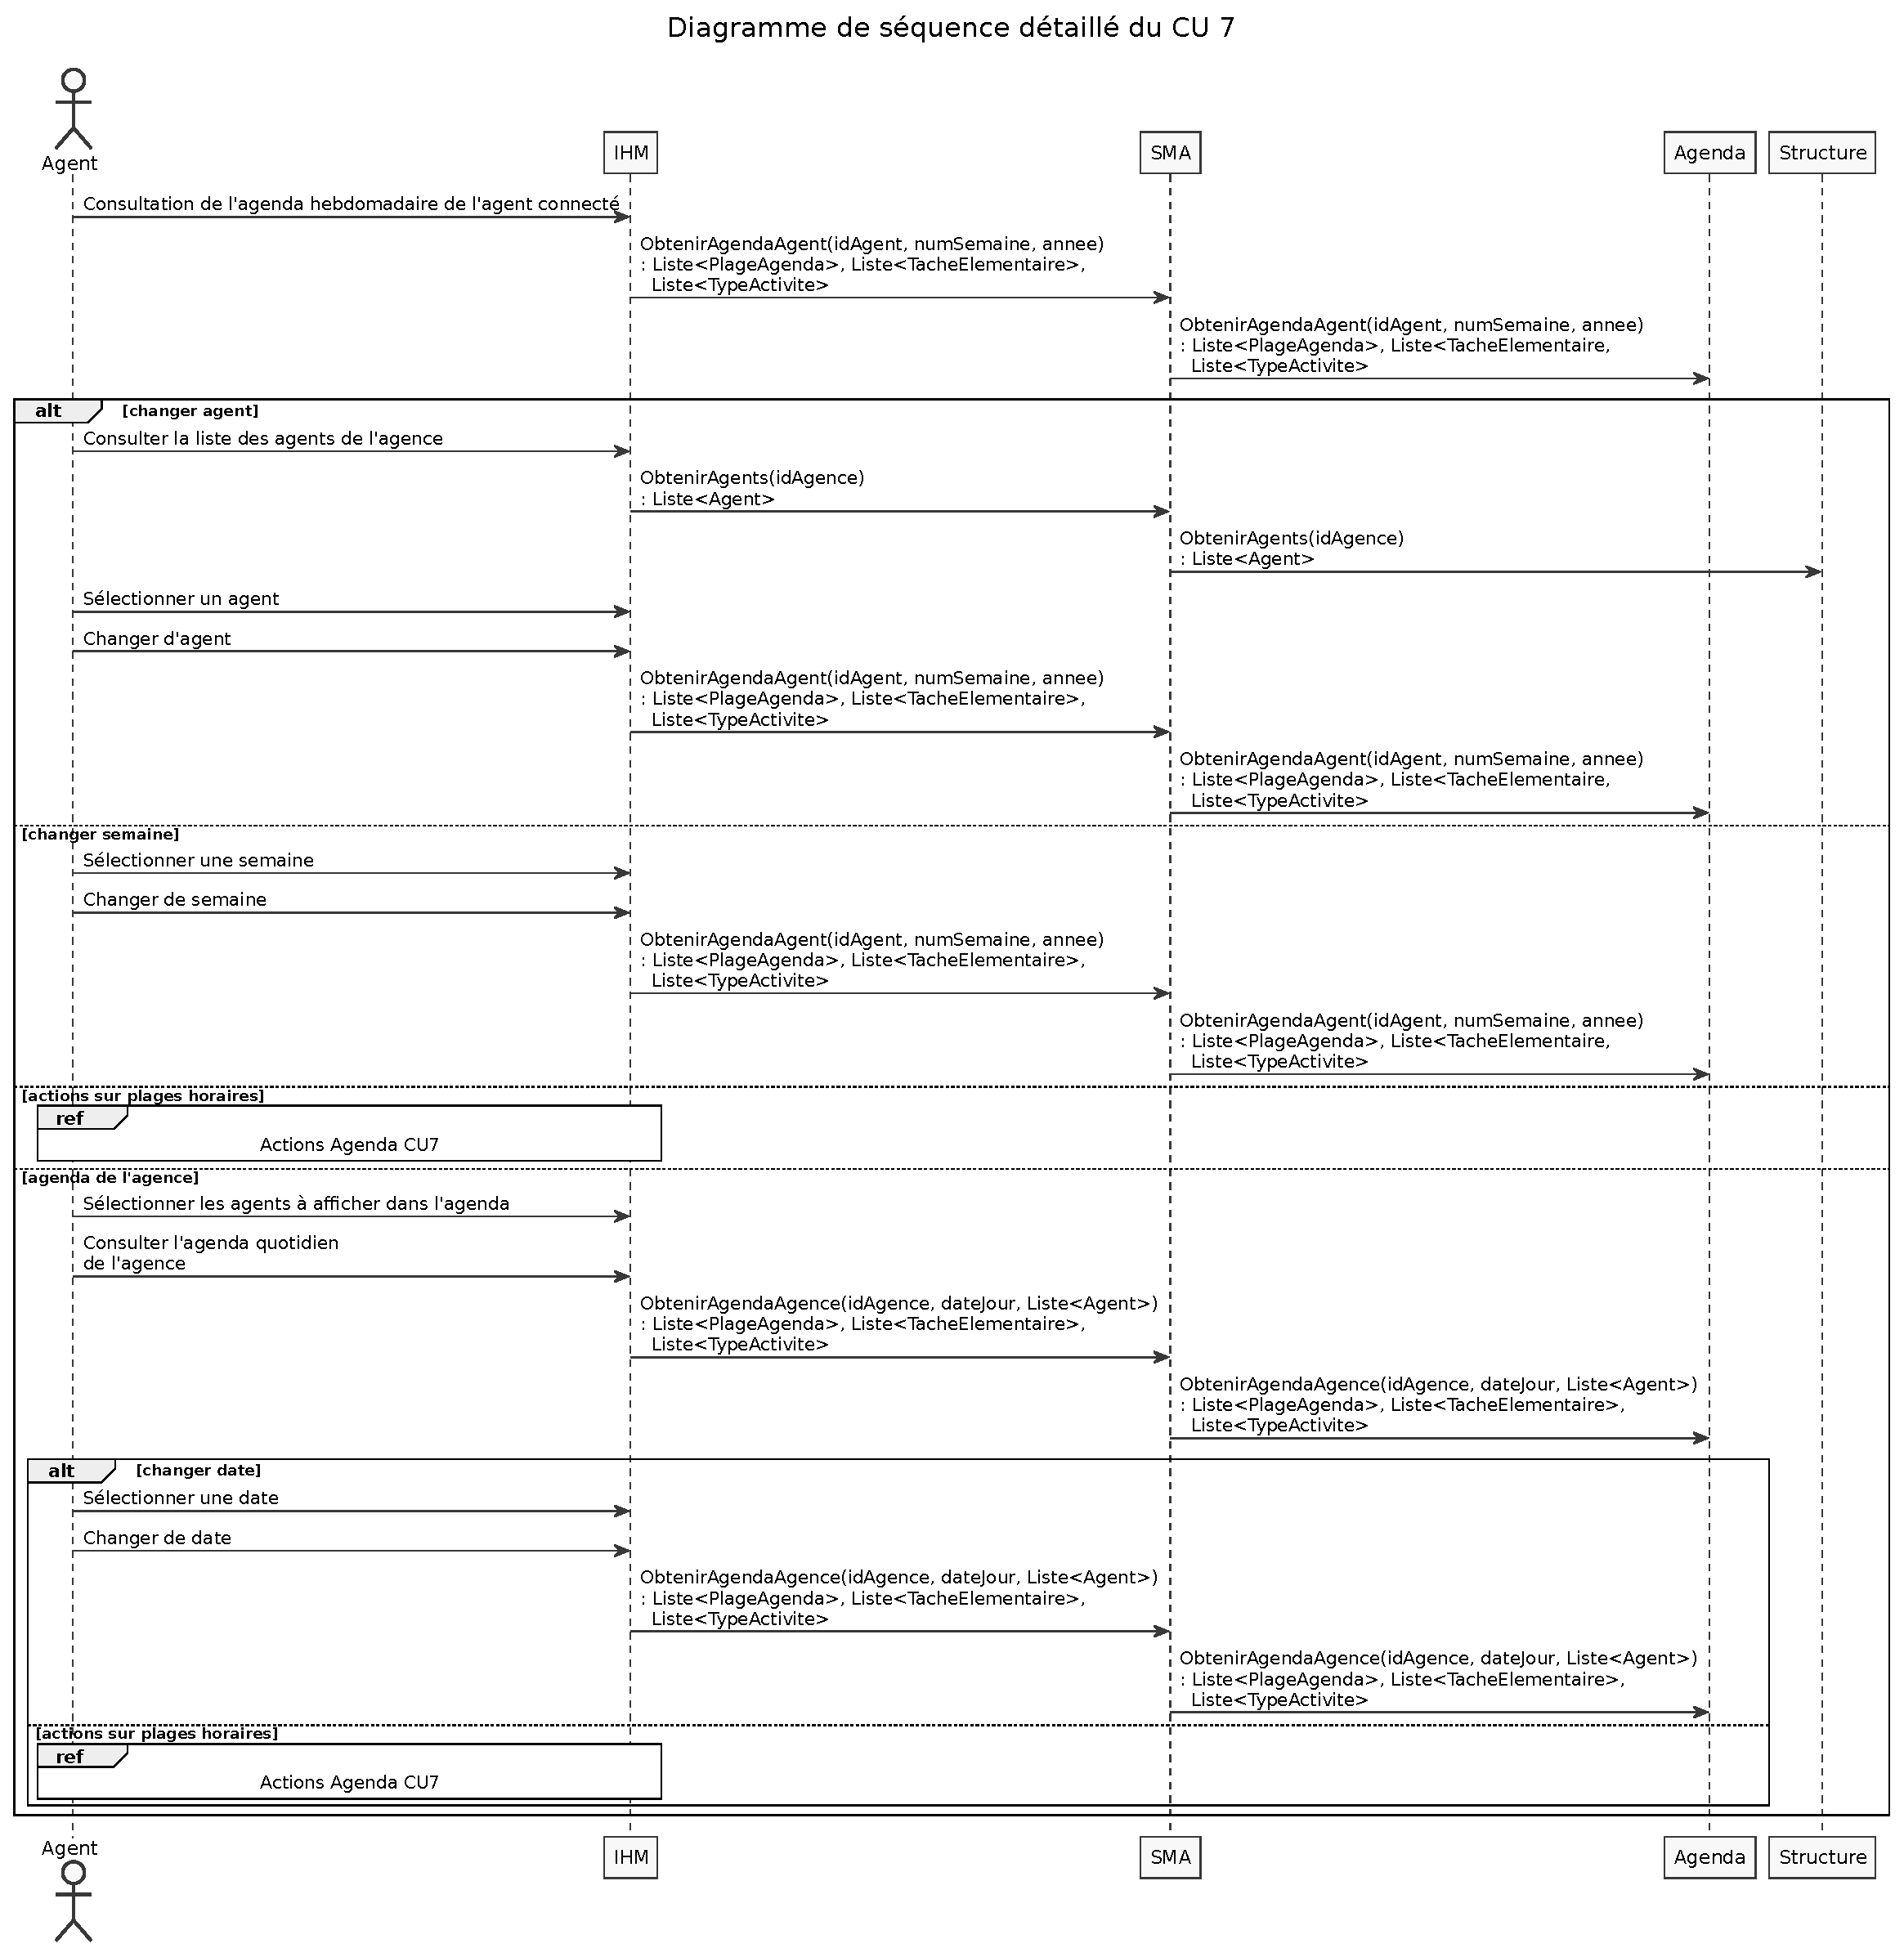
\includegraphics[height=12cm]{../report/figures/eps/DSD_CU7}}
    \end{frame}
    
    
        \begin{frame}{Diagramme de séquence détaillé - CU7}
    \adjustbox{width=1.1\textwidth, center, trim={0} {0} {0} {.55\height},clip}
  {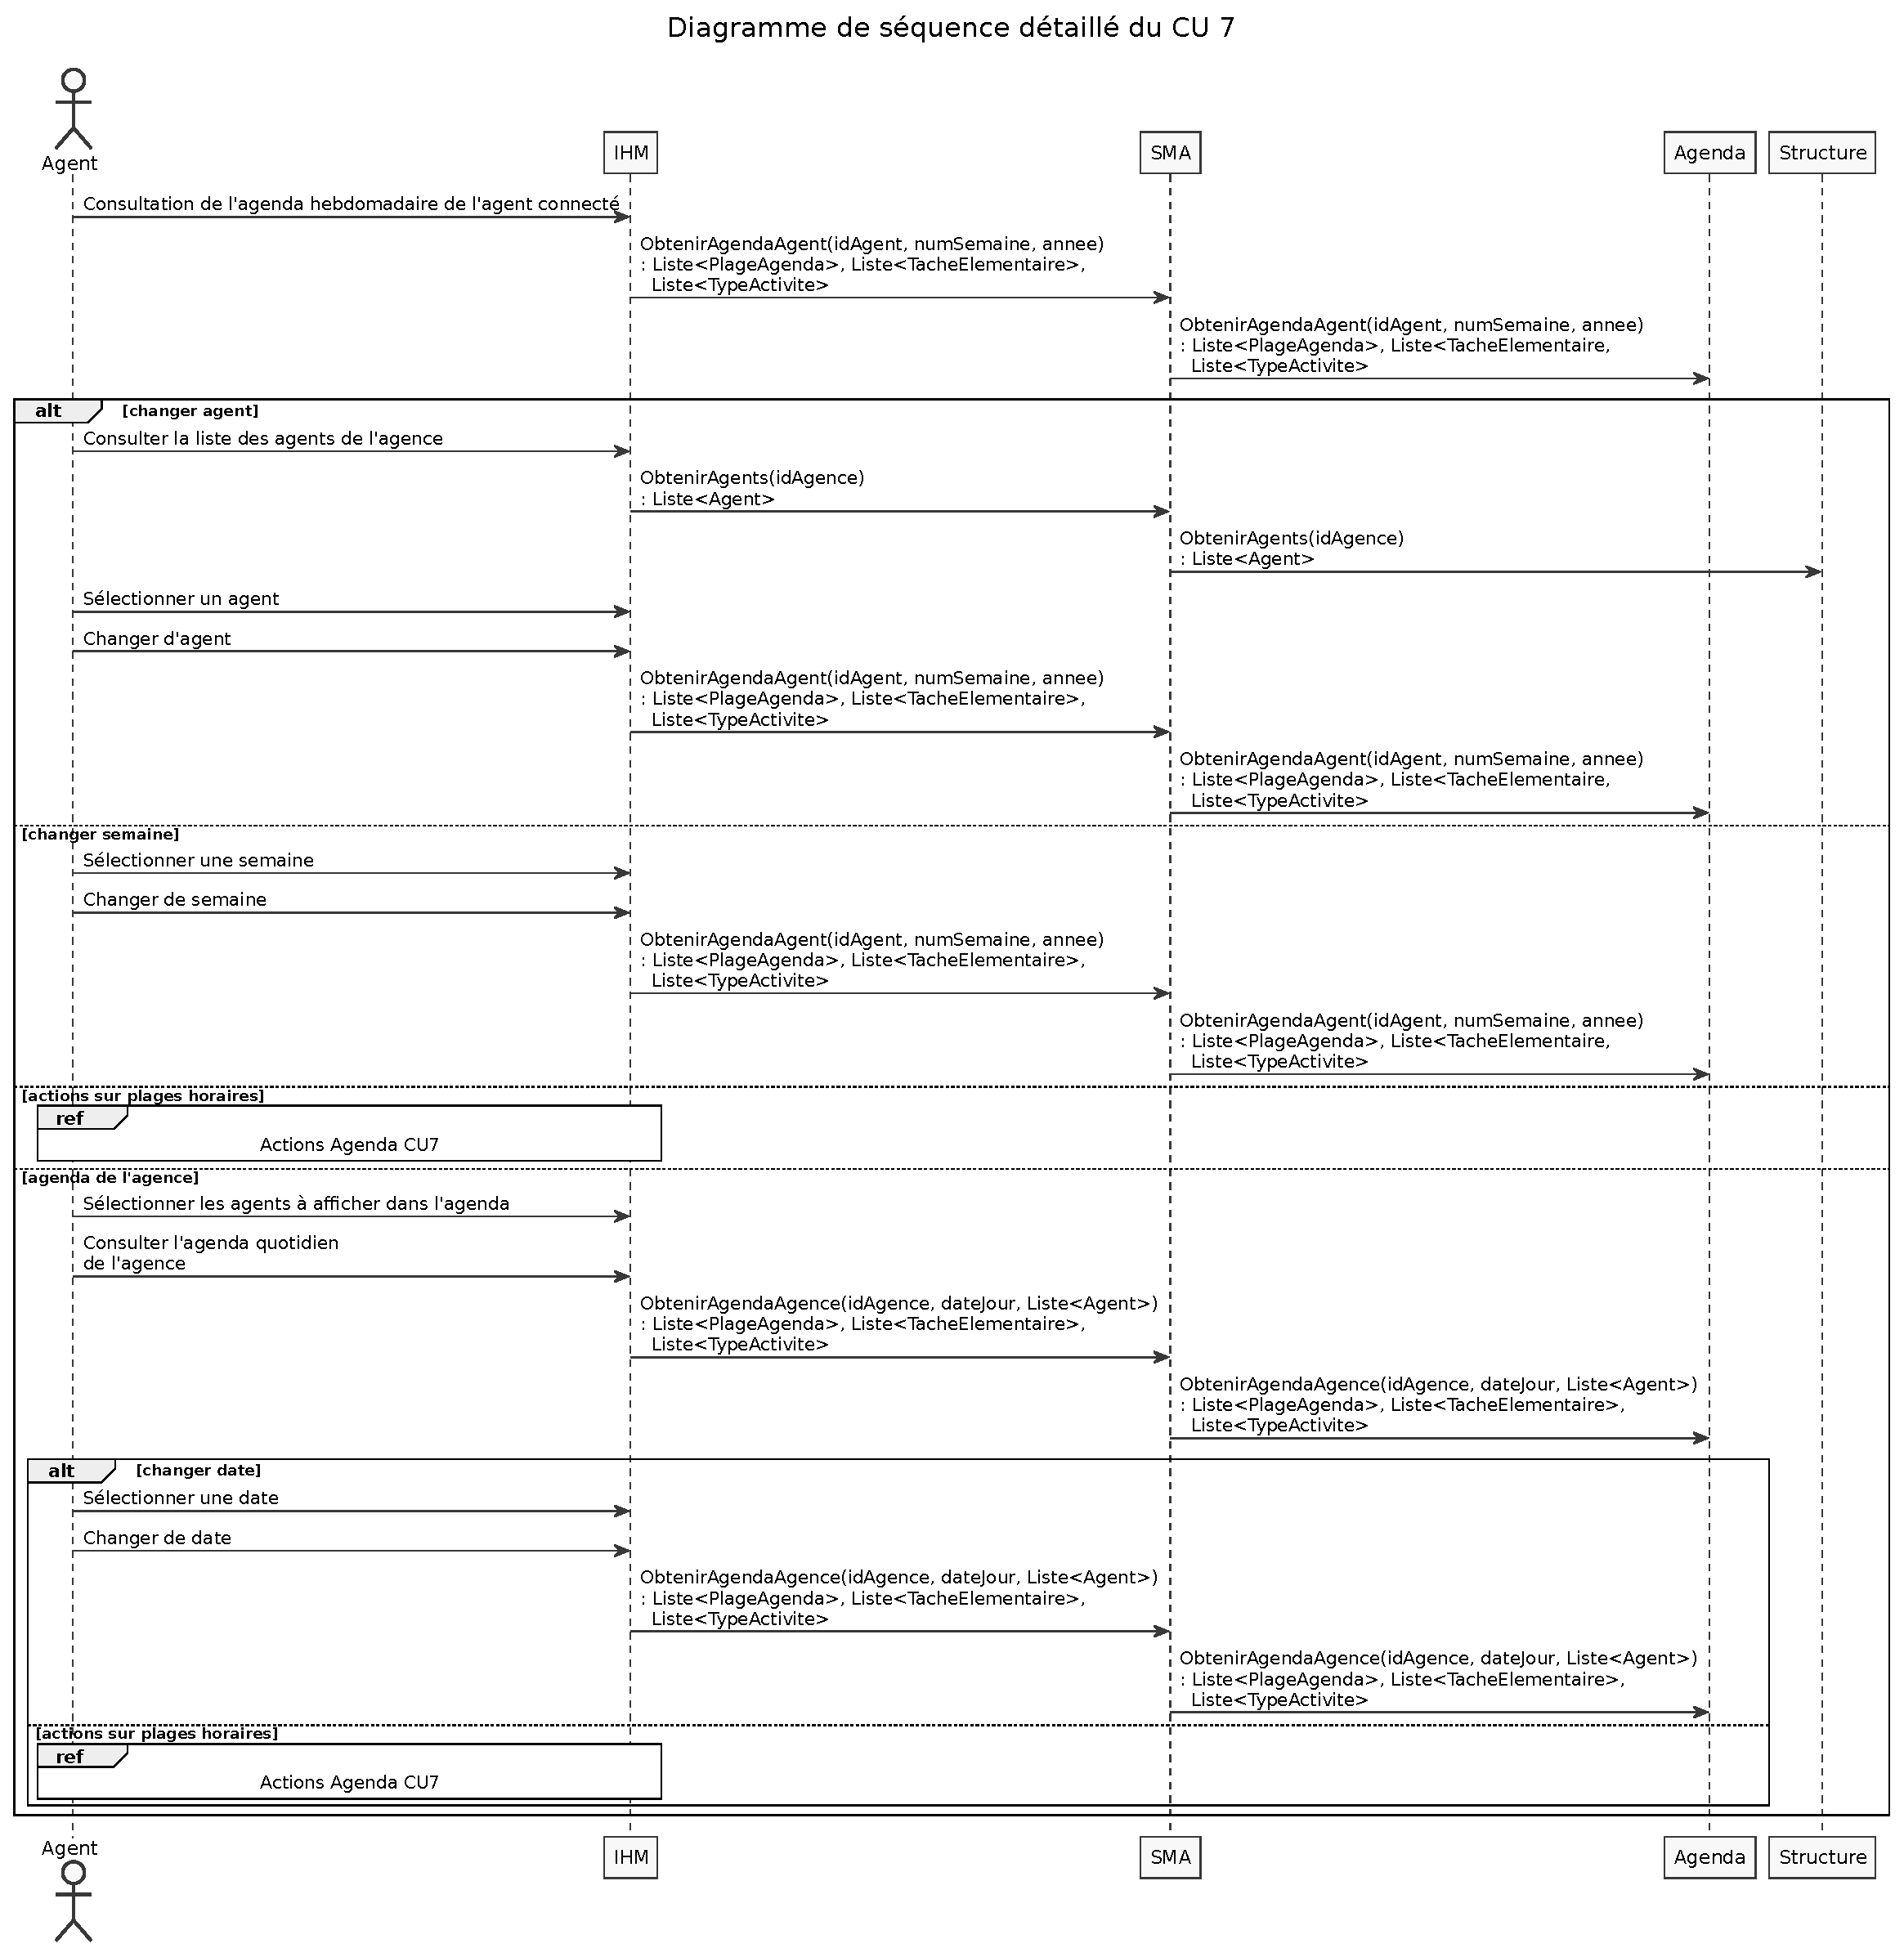
\includegraphics[height=12cm]{../report/figures/eps/DSD_CU7}}
    \end{frame}
    
    \begin{frame}{Diagramme de séquence détaillé - Action Agenda}
    
   \adjustbox{width=1.1\textwidth, center, trim={0} {.5\height} {0} {0},clip}%
  {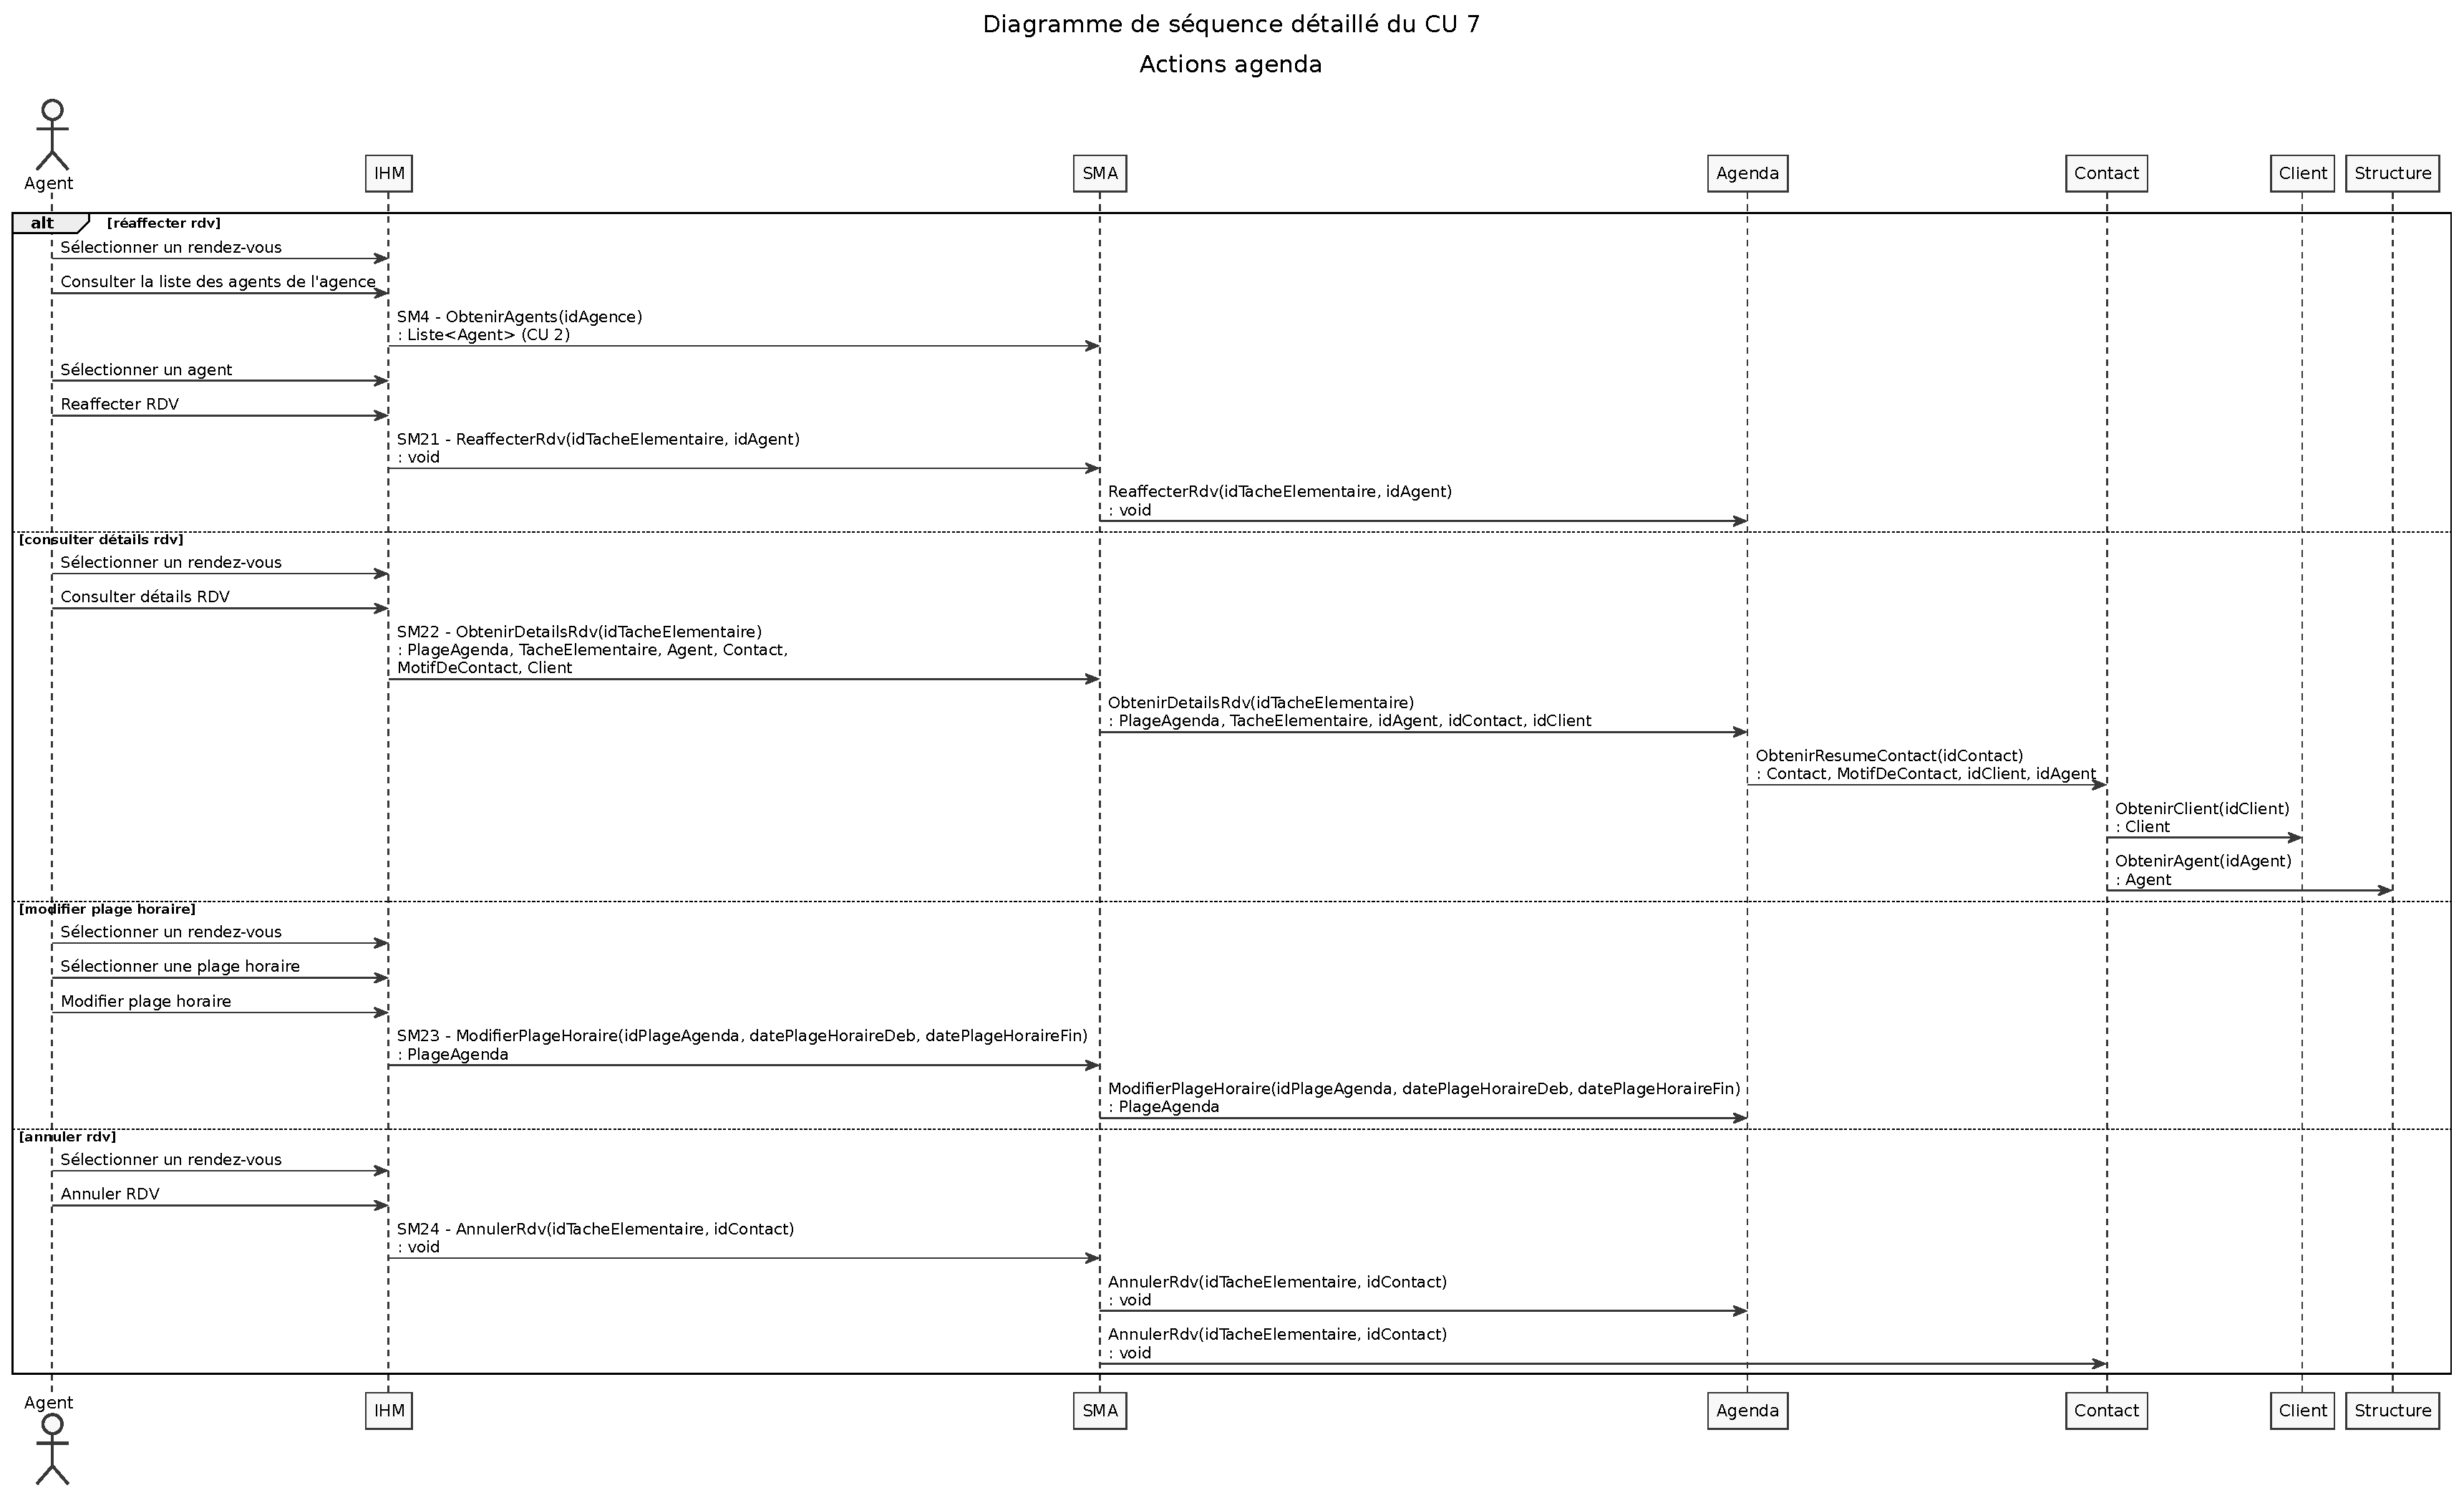
\includegraphics[height=12cm]{../report/figures/eps/DSD_CU7_ActionsAgenda}}

    \end{frame}
    
     \begin{frame}{Diagramme de séquence détaillé - Action Agenda}
    \adjustbox{width=1.1\textwidth, center, trim={0} {0} {0} {.5\height},clip}%
  {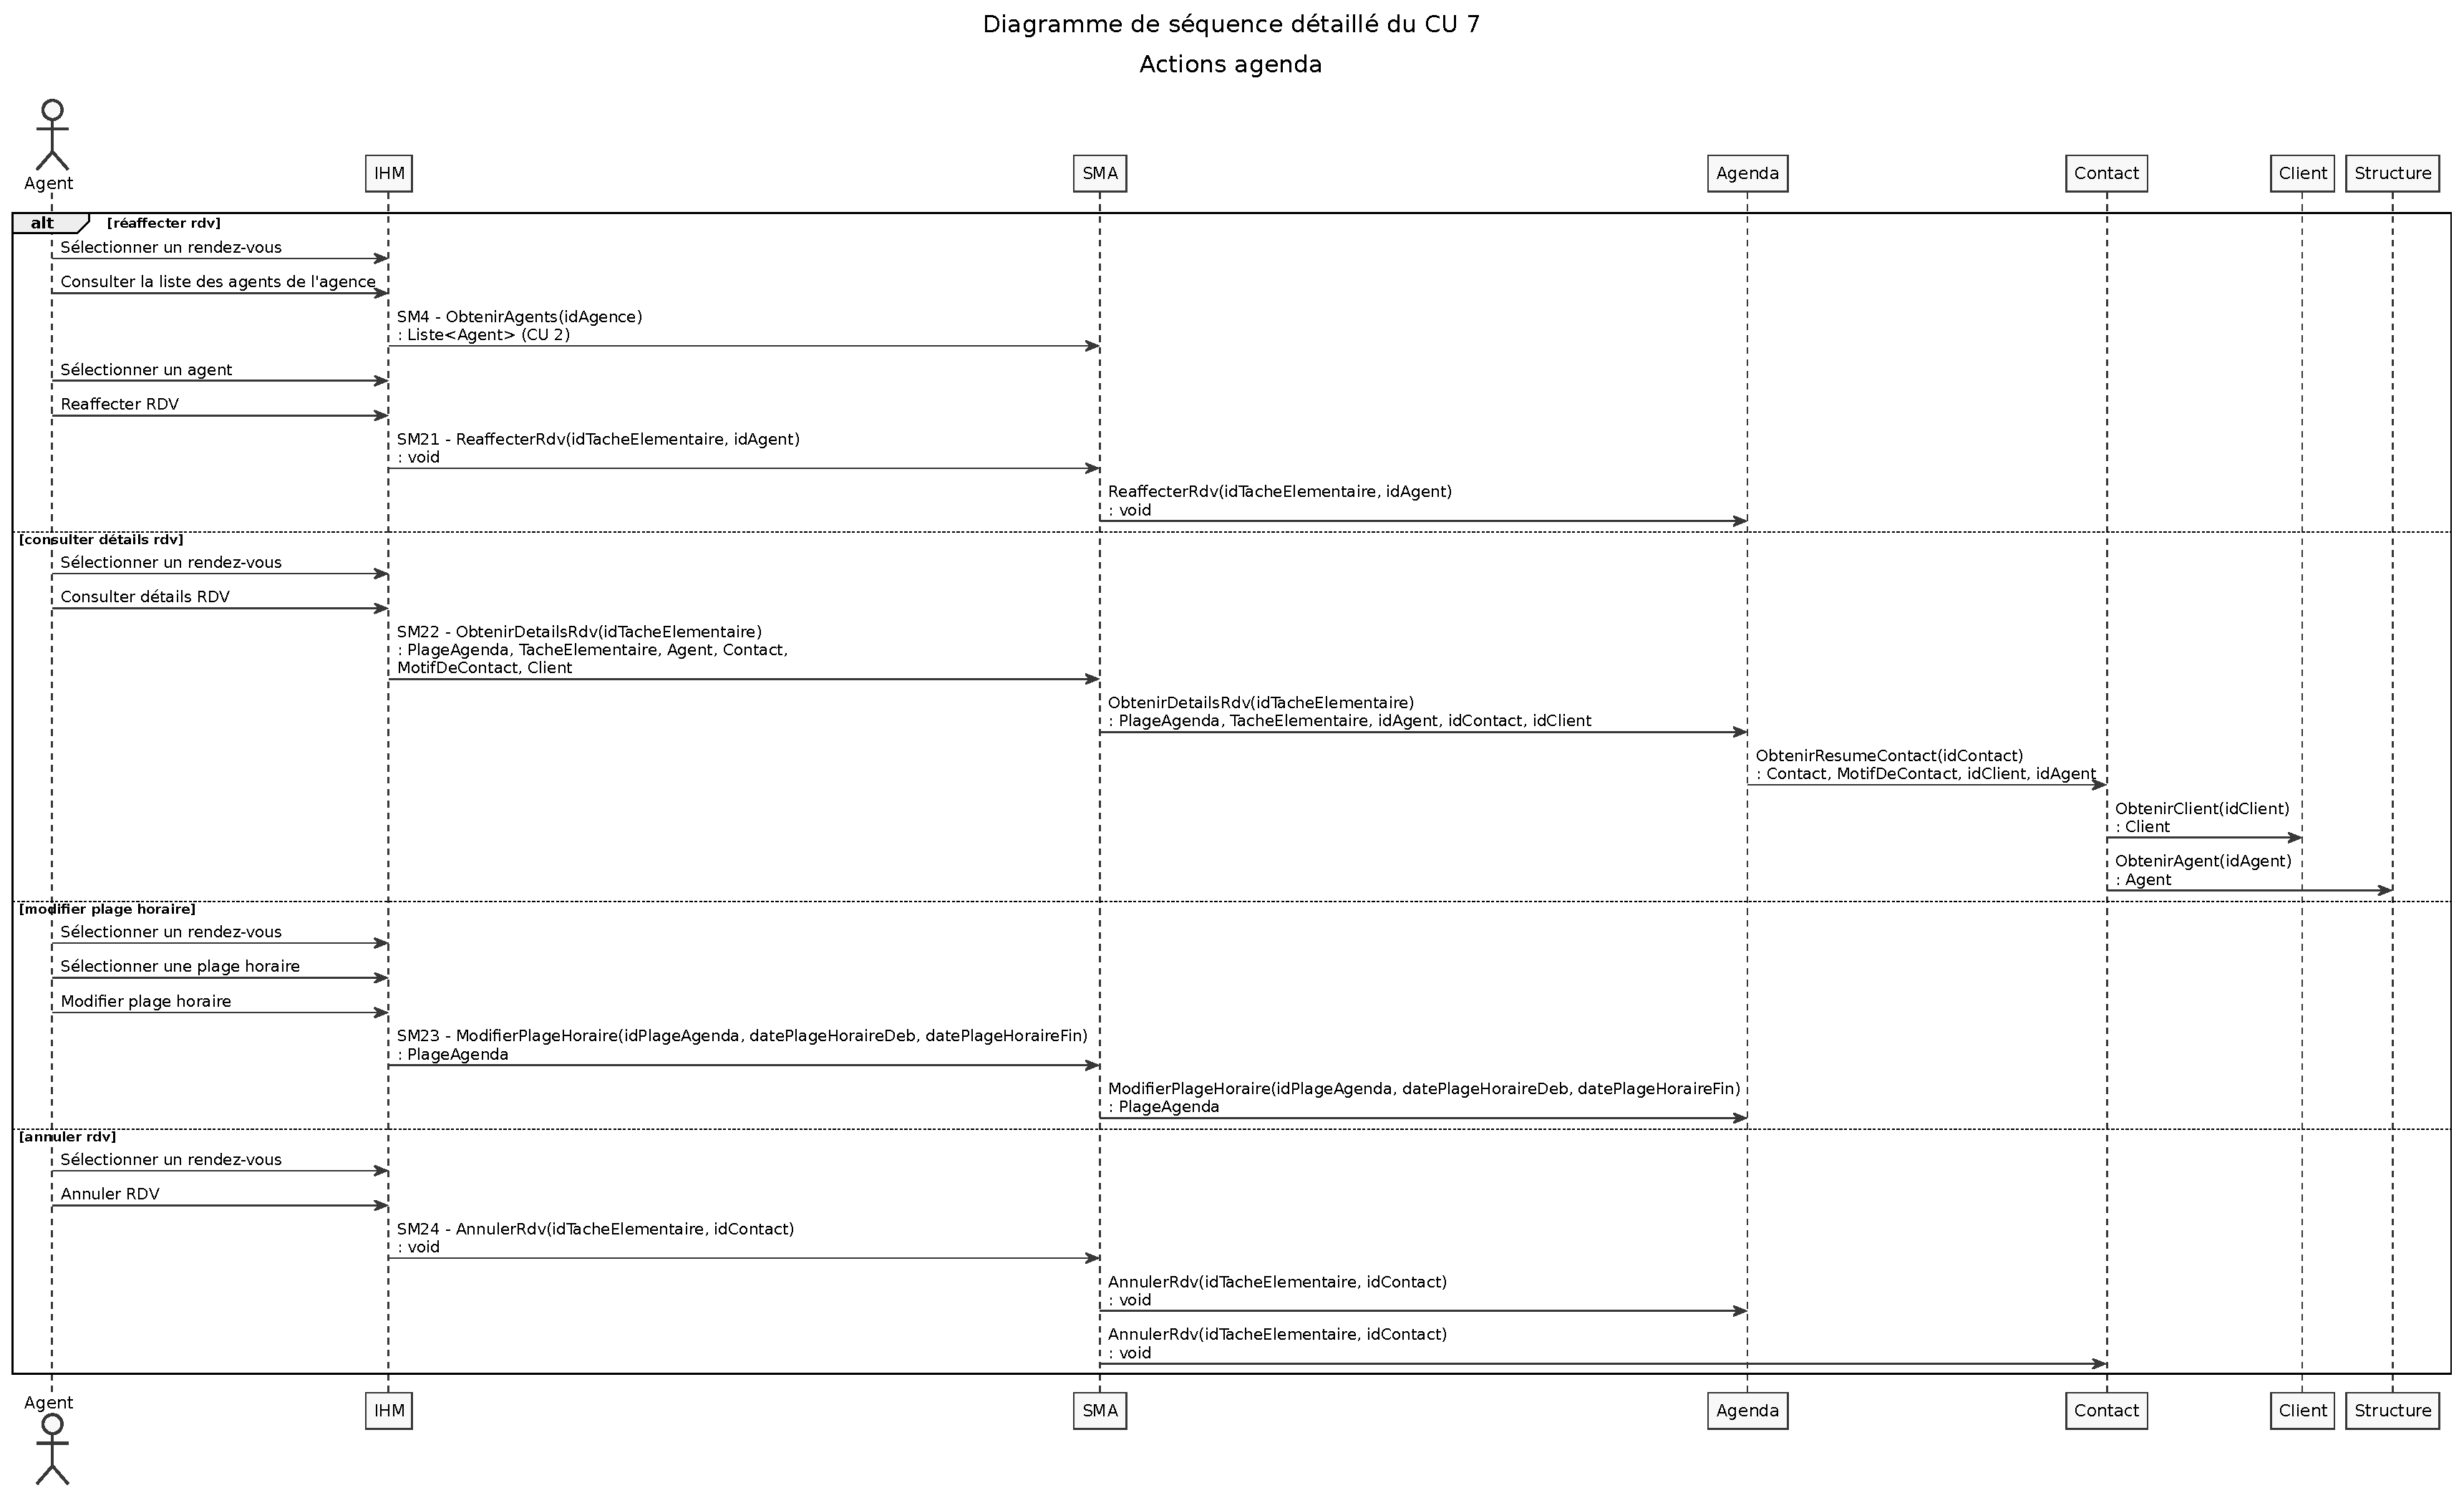
\includegraphics[height=12cm]{../report/figures/eps/DSD_CU7_ActionsAgenda}}
    \end{frame}
    
    
    \section{Diagramme de collaboration (Estelle)}
    \begin{frame}{Diagramme de collaboration}
\noindent\makebox[\textwidth]{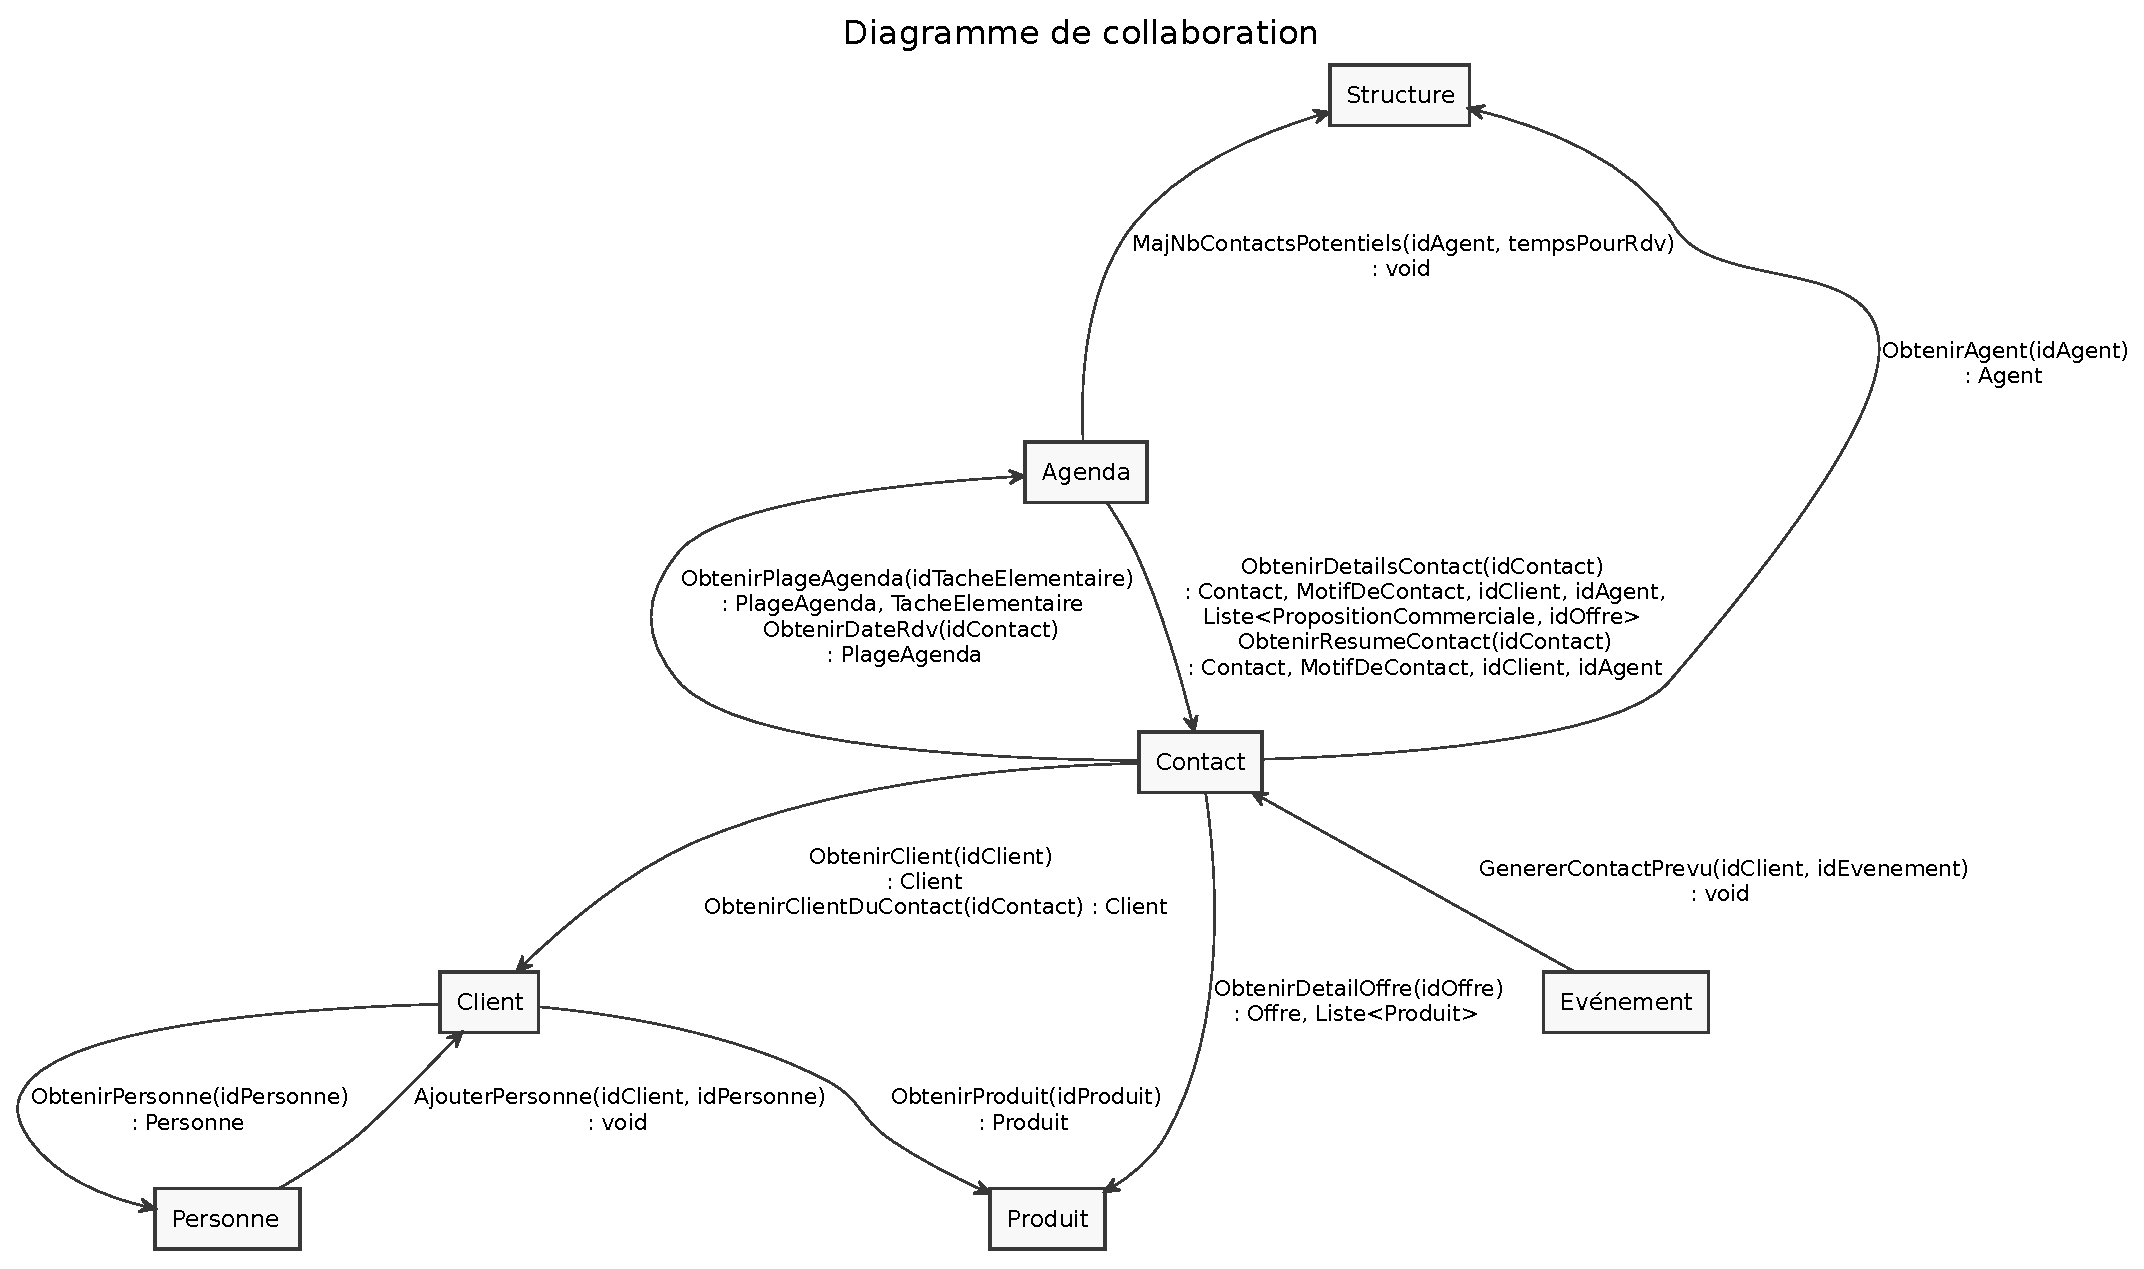
\includegraphics[height=5.5cm]{../report/figures/eps/collaboration}}
    \end{frame}
    
    \begin{frame}{Architecture}
\noindent\makebox[\textwidth]{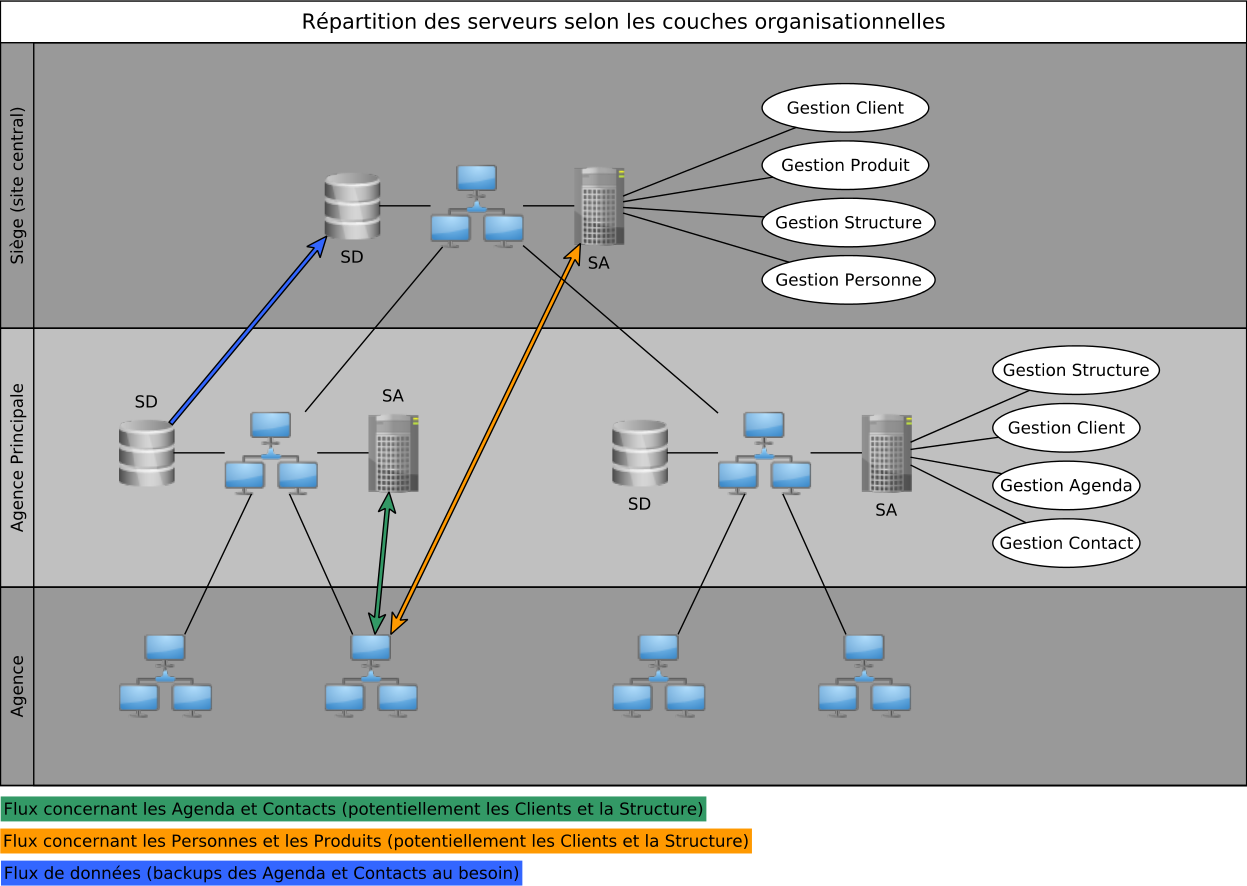
\includegraphics[height=8cm]{../report/figures/architectureServeurs.png}}
    \end{frame}
    
\section{2 SM + SOM (Pierre)}

\begin{frame}{SMA - Obtenir Détail Agent}
\begin{small}
\noindent Arguments en entrée
\begin{itemize}
\item idAgent 
\item numSemaine 
\item annee  \\
\end{itemize}

\noindent Sorties
\begin{itemize}
\item Liste<PlageAgenda>
\item Liste<TacheElementaires>
\item Liste<TypeActivite>
\end{itemize}
\end{small}

\end{frame}

\begin{frame}{SMA - Obtenir détails rdv}

\begin{small}
\noindent Arguments en entrée
\begin{itemize}
\item idPlageAgenda \\
\end{itemize}

\noindent Sorties
\begin{itemize}
\item PlageAgenda 
\item Agent
\item Contact
\item MotifDeContact 
\item Client 
\end{itemize}
\end{small}

\end{frame}
    
\begin{frame}{ObtenirDetailsRdv(idPlageAgenda)}

\noindent  Arguments en entrée
\begin{itemize}
\item idPlageAgenda  \\
\end{itemize}

\noindent Sorties 
\begin{itemize}
\item PlageAgenda 
\item idAgent  
\item idContact
\item idClient 
\end{itemize}

\end{frame}

\begin{frame}{ObtenirDetailsContact(idContact)}

\noindent  Arguments en entrée
\begin{itemize}
\item idContact \\
\end{itemize}

\noindent Sorties
\begin{itemize}
\item Contact  
\item MotifDeContact  
\item Liste<PropositionCommerciale, idOffre> 
\item idClient
\end{itemize}

\end{frame}

\begin{frame}{ObtenirClient(idClient)}

\noindent  Arguments en entrée
\begin{itemize}
\item idClient \\
\end{itemize}


\noindent Sorties
\begin{itemize}
\item Client
\end{itemize}

\end{frame}

\begin{frame}{ObtenirAgent(idAgent)}

\noindent  Arguments en entrée
\begin{itemize}
\item idAgent \\ 
\end{itemize}

\noindent Sorties
\begin{itemize}
\item Agent 
\end{itemize} 

\end{frame}

\begin{frame}{ObtenirDetailOffre(idOffre)}

\noindent  Arguments en entrée 
\begin{itemize}
\item idOffre \\
\end{itemize} 

\noindent Sorties
\begin{itemize}
\item Offre 
\item Liste<Produit>  
\end{itemize} 

\end{frame}
    
\begin{frame}{Bilan du projet}
  \begin{figure}
	\begin{tikzpicture}
      \begin{axis}[
        mbarplot,
        ylabel=Temps (Heures),
        axis y line=left,
        axis x line=bottom,
        xmin=0, xmax=5,
        ymin=0, ymax=40,
        xtick={1,2,3,4},
        xticklabels={Conception\\ d’ensemble,Conception\\ fonctionnelle\\ détaillée,Conception\\ applicative\\ détaillée,Architecture\\ technique},%<--Here
        xlabel style={yshift=-1cm},
        x tick label style={
            rotate=62,
            anchor=east,
            font=\footnotesize,
            align=right
        },
        width=\textwidth,
        height=7cm,
      ]

      \addplot plot coordinates {(1, 20) (2, 25) (3, 22.4) (4, 12.4)};
      \addplot plot coordinates {(1, 18) (2, 24) (3, 23.5) (4, 13.2)};

      \legend{Temps estimé, Temps passé}

      \end{axis}
    \end{tikzpicture}
  \end{figure}
\end{frame}

\end{document}
